\documentclass{article}


\usepackage{arxiv}

\usepackage[utf8]{inputenc} % allow utf-8 input
\usepackage[T1]{fontenc}    % use 8-bit T1 fonts
\usepackage{hyperref}       % hyperlinks
\usepackage{url}            % simple URL typesetting
\usepackage{booktabs}       % professional-quality tables
\usepackage{amsfonts}   
\usepackage{amsmath}% blackboard math symbols
\usepackage{nicefrac} 
\usepackage{graphicx}% compact symbols for 1/2, etc.
\usepackage{microtype}      % microtypography
\usepackage{lipsum}

\usepackage{titlesec}
\titlelabel{\thetitle.\quad}


\title{Performance Evaluation of Kervolutional Neural Networks for Automatic Satellite Images Analysis}


\author{
  Juan Sebastián Corredor\\%thanks{Use footnote for providing further
    %information about author (webpage, alternative
    %address)---\emph{not} for acknowledging funding agencies.} \\
  Department of Statistics\\
  Universidad Nacional de Colombia\\
  \texttt{jucorredorr@unal.edu.co} \\
  %% examples of more authors
   \And
   Camilo Pino\\%thanks{Use footnote for providing further
    %information about author (webpage, alternative
    %address)---\emph{not} for acknowledging funding agencies.} \\
  Department of Engineering\\
  Universidad Nacional de Colombia\\
  \texttt{camipinog@unal.edu.co} \\
  %% examples of more authors
   \And
  Iván Yesis Castellanos \\
  Department of Engineering\\
  Universidad Nacional de Colombia\\
  \texttt{iycastellanosm@unal.edu.co} \\
  %% \AND
  %% Coauthor \\
  %% Affiliation \\
  %% Address \\
  %% \texttt{email} \\
  %% \And
  %% Coauthor \\
  %% Affiliation \\
  %% Address \\
  %% \texttt{email} \\
  %% \And
  %% Coauthor \\
  %% Affiliation \\
  %% Address \\
  %% \texttt{email} \\
}

\begin{document}
\maketitle

\begin{abstract}
\small The main objective of this article is to adapt some architectures of CNNs to Convolutional Kernel Networks or Kervolutional Neural Networks and evaluate the performance of this models in a Kaggle Dataset of Satellite Images in order to classify and detect objects in it.
\end{abstract}


% keywords can be removed
\small \keywords{Kernel Methods \and Convolutional Neural Networks \and Computer Vision \and Image Segmentation}


\section{Project goal and scope}
% The very first letter is a 2 line initial drop letter followed
% by the rest of the first word in caps.
% 
% form to use if the first word consists of a single letter:
% \IEEEPARstart{A}{demo} file is ....
% 
% form to use if you need the single drop letter followed by
% normal text (unknown if ever used by the IEEE):
% \IEEEPARstart{A}{}demo file is ....
% 
% Some journals put the first two words in caps:
% \IEEEPARstart{T}{his demo} file is ....
% 
% Here we have the typical use of a "T" for an initial drop letter
% and "HIS" in caps to complete the first word.
Geospatial monitoring systems are one of the most important tools for decision-making around various issues such as illegal mining, deforestation, border patrolling, and environmental surveillance. Having timely and specific information regarding the dynamics of phenomena that can be measured by satellite images supports the decision-making process at different time scales, allowing the implementation of proactive/predictive strategies.\\
% You must have at least 2 lines in the paragraph with the drop letter
% (should never be an issue)

The automatic analysis of geospatial images supports the understanding of environmental phenomena, and human behavior, allowing to identify, prioritize, and explain events with high sensitivity and specificity in order to implement complete strategies for decision making.\\

In recent years, the performance of Artificial Intelligence techniques has presented a dramatic advance; This has allowed the emergence of innovative applications to problems in various areas, among them, the application of Kernel Methods and Deep Learning to Computer Vision problems stands out for promoting the creation of systems for decision making and classification, such as object recognition, classification of images by content and the development of autonomous vehicles.\\


In this sense, there are several reports in the scientific literature that describe the advantages of using classifiers based on Deep Learning in terms of the reduction in complexity of data pre-processing stages and obtaining quality measures at the state of the art level. This advance in the technique makes it possible to build systems for land use detection and classification for categories of interest without the need to establish reference frames, select spectral indexes or build decision trees manually. These components of the analysis are built and optimized automatically by the Deep Neural Network information and training integration system.\\
\subsection{Ideal situation}
Action upon sudden changes in the configuration of urban and rural geographic landscapes should be immediate and supported by the possibility of anticipating anomalous patterns over time. The detection of anomalies in the geographical landscape should be a semi-automatic process with the least frequency and the greatest coverage that the remote sensing equipment allows. Resources for the security of rural areas should be allocated optimally, providing timely responses and prioritizing incidents.\\

\subsection{Problem}
In Colombia, problems such as illegal crops, illegal mining, deforestation and border surveillance do not have automatic or manual information and analysis on short time scales (less than a week) over the entire national territory. At present, the ability to anticipate anomalous patterns over time in satellite images is limited by restrictions on the availability of specialized personnel, computational resources and information sources. Available commercial offers do not allow the use of remote sensing data from open sources with effectiveness and reasonable costs.\\

\subsection{Hypothesis}
Having tools based on Artificial Intelligence for automatic monitoring and early warning generation for problems with geospatial manifestation, would allow to prioritize incidents, optimize the allocation of resources, and establish proactive strategies for surveillance, control, and application of laws and norms over the national territory. It would allow the timely deployment of personnel and prioritization of actions on issues such as illegal mining, illegal crops, illegal occupation of national parks, deforestation, fires, floods, and border surveillance according to a mapping and diagnosis processes for the identification and targeting of environmental and human phenomena.\\

\subsection{Goal}

In this project we explore the combination of kernel methods and deep learning techniques for the automatic classification of geospatial images.\\

We aim to take advantage of the strengths of deep convolutional neural networks and their translation into convolutional kernel networks. This combination has the potential to improve existing performance on the task of land cover classification, and object detection in remote sensing imagery.

\subsection{Scope and Literature Review}
We plan to use a publicly available dataset on image feature detection. This dataset must have an existing baseline based on manual and automatic labeling.\\

\subsubsection{Convolutional Neural Networks and Image Classification and Detection}

The availability of satellite imagery for every corner of the planet has enabled several applications that could not be feasible with other types of observation techniques. At the same time, the volume of continuously updated and historical data represents a challenge for the analysis, which can not be possible without automation \cite{maggiori2016convolutional}.\\

Among  image processing tasks in geospatial analysis, object detection and classification is one of the most common steps. Object detection and classification allows to quantify terrain features with significance in a particular problem for each unit of analysis. At its turn, this measurements are used as inputs for different models, with applications in diverse domains such as environmental, industrial, agricultural, epidemiological, national security, and economic planning \cite{maggiori2016convolutional}.\\

The state of the art in image processing techniques for object detection and classification makes use of convolutional neural networks. These type of network, originally proposed in 1980 \cite{fukushima1980neocognitron}, had a tremendous growth of use for several image processing in the 2000s. Factors that contribute to their widespread use are the currently available computing capability (Graphical Processing Units), existence of large enough datasets for training, and good performance for diverse tasks \cite{liu2017survey}.\\

Another artificial intelligence techniques that have been used widely for computer vision are the kernel methods  \cite{LampertKernel} which are based on a implicit projection of the images into a high dimensional Hilbert space, where the data can be linearly related. One of the  main advantages of kernel methods over neural networks is the possibility of include knowledge about the field, however, the main disadvantage is the lack of scalability to large datasets.\\

\subsubsection{Theory and Implementation}

Ideally, strategies that combine the advantages of kernel methods and neural networks can be very useful in computer vision field. Recently, some advances about this have been made with the development of Convolutional Kernel Networks (CKN) \cite{NIPS2014_5348} which are based on a deep architecture of kernel machines instead of a shallow one. The main idea is to put kernel functions as layers in a network and analyze images in a convolutional way, i.e. through patches in each layer.\\

Convolutional Kernel Networks have showed good performance for computer vision tasks compared to Convolutional Neural Networks. In fact, it can be shown that a CNN architectures can be translated into a CKN ones defining a similar translational invariations by the concatenation of convolutional layers \cite{DBLP:journals/corr/abs-1904-03955}.\\ 

We will use available implementations of the baseline methods and Kervolutional Neural Networks, constructed in \cite{DBLP:journals/corr/abs-1904-03955}. Convolutional operator is defined as
\begin{align*}
    f(x) &= x \oplus w
\end{align*}
where $x,w \in \mathbb{R}^n$. Note that the $i$-th element of the convolution output $f(x)$ is calculated as:
\begin{align*}
    f_i(x) &= <x_{(i)}, w>
\end{align*}
where $<\cdot,\cdot>$ is the inner product of two vectors and $x_{(i)}$
is the \textit{circular} shift of $x$ by $i$ elements. \cite{DBLP:journals/corr/abs-1904-03955} defines the index $i$
started from $0$. The kervolution output $g(x)$ is defined as
\begin{align*}
    g(x)&= x \otimes w 
\end{align*}
where $\otimes $ is the kervolutional operator. Specifically, the $i$-th
element of $g(x)$ is defined as:
\begin{align*}
    g_i(x) &=  <\phi(x_{(i)}),\phi(w)>
\end{align*}
where $\phi: \mathbb{R}^n \to \mathbb{R}^d$ ($d \gg n$) is a non-linear mapping
function. The key of this idea is to extract features in a high and more complex dimensional space and avoiding the extra computational complexity via the \textit{Kernel Trick} i.e:
\begin{align*}
    <\phi(x_{(i)}),\phi(w)> &= k(x_{(i)}, w)
\end{align*}
where $k: \mathbb{R}^n \times \mathbb{R}^n \to \mathbb{R}$ is the predefined kernel whose, as establishes \cite{DBLP:journals/corr/abs-1904-03955},
complexity is normally of $O(n)$, equal to the complexity of the convolutional inner product; contrary to other non-linear convolutional algorithms with $O(n\cdot \log(n))$ or even $O(n^2)$ complexity.\\
\\
As a matter of fact, \cite{DBLP:journals/corr/abs-1904-03955} found that the kervolution operator is equivariant to translation (see Theorem 3.1), which means that maintains one the greatest and important properties of the convolutional operator.\\
\\
 \textbf{The non-linearity of ReLU and MaxPooling.} Most of non-linearity in CNNs are the activation (generally ReLU) and the MaxPooling layers. Using KNNs (Kervolution Neural Networks), we do not need it since we already are using non-linear mapping functions. \cite{DBLP:journals/corr/abs-1904-03955} proposes remove all the activation layers and change the MaxPooling layers to AvgPooling (that is a linear pooling). 

\section{Case study}

We took two case studies as references for the methodology, datasets, and utility aspects for this project: the methodology technical report of the United Nations Office on Drugs and Crime (UNODC) Sistema Integrado de Monitoreo de Cultivos Ilícitos (SIMCI), which is the most authoritative source of illegal crops, and illegal minery for Colombia making use of geospatial analysis \cite{Nevada2017MetodologiaCoca}; and the Kaggle competition "Dstl Satellite Imagery Feature Detection" which was proposed around a feature detection dataset \cite{kaggledstl2017}.\\

The UNODC SIMCI report \cite{UNODC2017Monitoreo2017} makes use of a traditional methodology, in which additional data sources are used as manual reference only. They defined a decision tree that allowed to select a pool of candidate zones for illicit crops. This pool was further refined, and the report was made by augmenting the manually curated data with historical records.\\

The Kaggle competition on object detection and classification launched in 2017, given its online nature and the technological tools that allow the sharing and reproducibility of solutions, is associated with a wide variety of solutions for the proposed problem. The dataset (which we chose to use in this project and is described in the following section) is publicly available, as well as solutions using different techniques, from SVMs to Convolutional Neural networks. This case study is ideal because it has several performance baselines.

\section{Training data set}

For the purposes of the competition \cite{kaggledstl2017}, Dstl provides 1km x 1km satellite images in both 3-band and 16-band formats, with the goal for detection and classification of objects found in these regions. The satellite that took this images is WorldView-3. The 3-band images are RGB natural color omages. The 16-band images contain additional spectral information. These images are provided in the GeoTiff format.\\

There are 10 different object types annotated in the dataset:
\begin{itemize}
    \item[1.]{Buildings}
    \item[2.]{Miscellaneous man-made structures}
    \item[3.]{Roads}
    \item[4.]{Tracks}
    \item[5.]{Trees}
    \item[6.]{Crops}
    \item[7.]{Waterways}
    \item[8.]{Standing water}
    \item[9.]{Large vehicles}
    \item[10.]{Small vehicles}
\end{itemize}

These objects are described by a polygon and a type in GeoJSON and WKT formats. The original coordinates of the images are replaced by a [0, 1] coordinate system. The dataset size is 20GB.

\section{Data pre-processing}
Baseline CNN training: The training dataset consists of 450 1km x 1km RGB images, of which only 25 are annotated with different features. The images and annotations were received in TIFF and CSV format.\\

The annotations contain multiple polygons per image and object type combinations, these polygons represent different instances of the object on the image. Each polygon is transformed into a mask in order to extract the corresponding pixels to be sampled in the neural network training process.\\

The values in the images range according to the satellite sensor, and thus, we transform them to a scale in which they could be visualized. In order to do this, the higher and lower 2\% values  of the range of each sensor in each image are used to scale the values.\\

\section{Neural Network Approach}
As mentioned above, we decided to use the mapping suggested in \cite{DBLP:journals/corr/abs-1904-03955}, that it is:
\begin{center}
 \begin{tabular}{ |c|c|} 
 \hline
 CNNs & KNNs \\  
 \hline
 \hline
Convolutional Layer & Kervolutional Layer (Polynomial, Gaussian) \\
ReLU (or other activation) & - \\
MaxPooling & AvgPooling \\
UpSampling & - \\ 
\hline
\end{tabular}
\end{center}
On the otherside, we used Tensorflow-Keras implementation and use the kervolution operator code implemented by $\cite{Charles2013}$ in Github in which it can be found the Polynomial and Gaussian Kernels.\\
\\
As baseline, a CNN with reported best performance on the Dstl dataset was used, its architecture is based on UNET, an architecture originally proposed for biomedical image segmentation, shown in the following figure.

\begin{figure}[h!]
    \center
    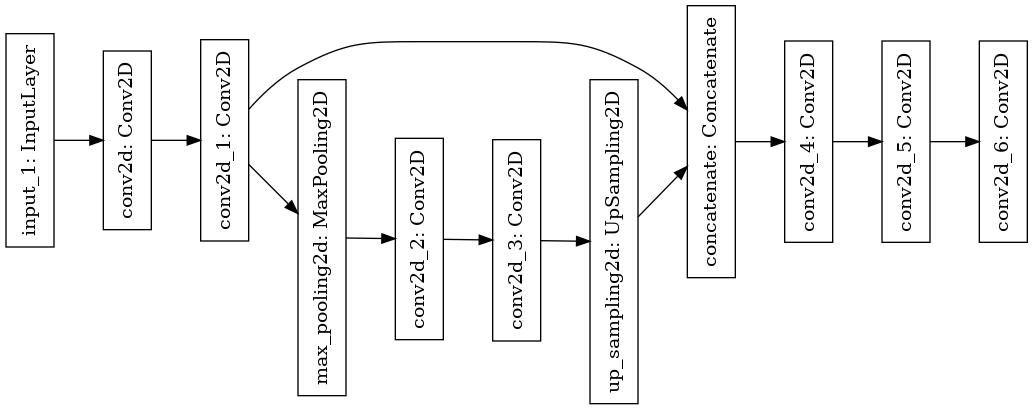
\includegraphics[width=0.65\linewidth]{Images/model.png}
    \caption{Baseline CNN - UNET.}
\end{figure}

This architecture consists of two paths of convolutions, a contracting path to capture context, and an expanding path to allow localization. These are presented in the architecture diagram as the two different paths which are merged at the Concatenate layer. This concatenation is further processed with convolutional layers in order to produce the output.\\

The strategy of UNET for capturing local, small changes, while also considering a broader context can also be useful for detecting objects in geospatial images, in which taking into account the broader characteristics of the image could help to precisely classify subtle changes.\\

This problem corresponds to a multiclass classification problem, for that purpose, the output of the last layer of the neural network uses a sigmoid (that won't be removed in the KNNs) activation function, with a neuron for each output type. The loss uses as metric the average of the Jaccard coefficient for the 10 classes.\\

\section{Results}

We obtained the source code for the best performing solution of the challenge, and adapted it to run in a recent version of Tensorflow. For performance and computational resource consumption of the model, some modifications had to be done in order to be able to run the experiment. These ranged from experimenting with different batch sizes and data loading strategies.

\begin{center}
 \begin{tabular}{ |c|c|c|c| } 
 \hline
 \multicolumn{4}{|c|}{UNET CNN Metrics}\\
 \hline
 \hline
 Id & Jaccard & Threshold & Object Description \\  
 \hline
 \hline
$1$ & $0.7009$ & $0.1$ & \scriptsize Buildings- Large Building, Residential, Non-Residential, Fuel Storage Facility, Fortified Building\\
\hline
$2$ & $0.7355$ & $0.1$ & \scriptsize Misc. Manmade Structures\\
\hline
$3$ & $0.8829$ & $0.1$ & \scriptsize Road\\
\hline
$4$ & $0.6169$ & $0.1$ & \scriptsize Track- Poor/Dirt/Cart Track, Footpath/Trail\\
\hline
$5$ & $0.5530$ & $0.2$ & \scriptsize Trees- Woodland, Hedgerows, Groups of Trees, Standalone Trees\\
\hline
$6$ & $0.5080$ & $0.4$ & \scriptsize Crops- Contour Ploughing/Cropland, Grain (Wheat) Crops, Row (Potatoes, Turnips) Crops\\
\hline
$7$ & $0.9729$ & $0.1$ & \scriptsize Waterway\\
\hline
$8$ & $0.9840$ & $0.1$ & \scriptsize Standing Water\\
\hline
$9$ & $0.9862$ & $0.1$ & \scriptsize Vehicle Large- Large Vehicle (e.g. Lorry, Truck, Bus), Logistics Vehicle\\
\hline
$10$ & $0.9458$ & $0.1$ & \scriptsize Vehicle Small- Small Vehicle (Car, Van), Motorbike\\
\hline
\end{tabular}
\end{center}

The obtained average Jaccard similarity is 0.7886, which is comparable to the announced.\\
\\
We changed every convolutional layer by a polynomial kervolutional layer of degree 2 and didn't obtain good results at all: The training accuracy lower than 0.4 for 10 epochs and a Jaccard Index of approximately 0.07, which was very disappointing.

\begin{center}
 \begin{tabular}{ |c|c|c|c| } 
 \hline
 \multicolumn{4}{|c|}{UNET KNN Metrics}\\
 \hline
 \hline
 Id & Jaccard & Threshold & Object Description \\  
 \hline
 \hline
$1$ & $0.0720$ & $0.0$ & \scriptsize Buildings- Large Building, Residential, Non-Residential, Fuel Storage Facility, Fortified Building\\
\hline
$2$ & $0.0722$ & $0.0$ & \scriptsize Misc. Manmade Structures\\
\hline
$3$ & $0.0723$ & $0.0$ & \scriptsize Road\\
\hline
$4$ & $0.0724$ & $0.0$ & \scriptsize Track- Poor/Dirt/Cart Track, Footpath/Trail\\
\hline
$5$ & $0.0726$ & $0.0$ & \scriptsize Trees- Woodland, Hedgerows, Groups of Trees, Standalone Trees\\
\hline
$6$ & $0.0726$ & $0.0$ & \scriptsize Crops- Contour Ploughing/Cropland, Grain (Wheat) Crops, Row (Potatoes, Turnips) Crops\\
\hline
$7$ & $0.0728$ & $0.0$ & \scriptsize Waterway\\
\hline
$8$ & $0.0729$ & $0.0$ & \scriptsize Standing Water\\
\hline
$9$ & $0.0730$ & $0.0$ & \scriptsize Vehicle Large- Large Vehicle (e.g. Lorry, Truck, Bus), Logistics Vehicle\\
\hline
$10$ & $0.0730$ & $0.0$ & \scriptsize Vehicle Small- Small Vehicle (Car, Van), Motorbike\\
\hline
\end{tabular}
\end{center}
\newpage
Having this, we decide to change the architecture of the NN to the following:
\begin{figure}[h!]
    \center
    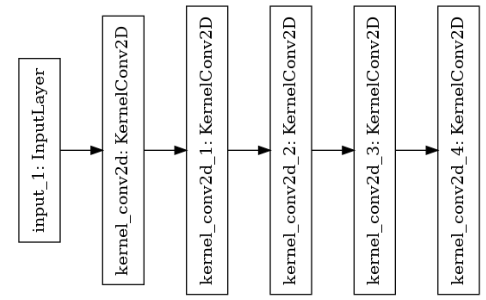
\includegraphics[width=0.35\linewidth]{Images/SEQKNN.png}
    \caption{Sequential KNN.}
\end{figure}

Unfortunately, the results were equally bad with respect to the UNET KNN:

\begin{center}
 \begin{tabular}{ |c|c|c|c| } 
 \hline
 \multicolumn{4}{|c|}{Sequential KNN Metrics}\\
 \hline
 \hline
 Id & Jaccard & Threshold & Object Description \\  
 \hline
 \hline
$1$ & $0.0719$ & $0.0$ & \scriptsize Buildings- Large Building, Residential, Non-Residential, Fuel Storage Facility, Fortified Building\\
\hline
$2$ & $0.0721$ & $0.0$ & \scriptsize Misc. Manmade Structures\\
\hline
$3$ & $0.0723$ & $0.0$ & \scriptsize Road\\
\hline
$4$ & $0.0724$ & $0.0$ & \scriptsize Track- Poor/Dirt/Cart Track, Footpath/Trail\\
\hline
$5$ & $0.0726$ & $0.0$ & \scriptsize Trees- Woodland, Hedgerows, Groups of Trees, Standalone Trees\\
\hline
$6$ & $0.0725$ & $0.0$ & \scriptsize Crops- Contour Ploughing/Cropland, Grain (Wheat) Crops, Row (Potatoes, Turnips) Crops\\
\hline
$7$ & $0.0727$ & $0.0$ & \scriptsize Waterway\\
\hline
$8$ & $0.0728$ & $0.0$ & \scriptsize Standing Water\\
\hline
$9$ & $0.0730$ & $0.0$ & \scriptsize Vehicle Large- Large Vehicle (e.g. Lorry, Truck, Bus), Logistics Vehicle\\
\hline
$10$ & $0.0730$ & $0.0$ & \scriptsize Vehicle Small- Small Vehicle (Car, Van), Motorbike\\
\hline
\end{tabular}
\end{center}
We wanted to try with different kernels (such a polynomial of other degrees and the gaussian) but because all the time that it took us to adapt the existing code about kervolution we could not test anymore models.
\section{Conclusions and Further Work in KNNs}
It is difficult to validate uses and performance of new kinds of layers, beacuse the implementation of these layers in tools like tensorflow and pythorch is tricky.
Therefore, assessing the real performance of kervolutional neural networks requires further work that we couldn't do must to the time used in the construction of the kervolutional layers.\\
\\
On the other hand, preprocessing of satellite images requires special computer configurations (64GB just for training and test data). New versions of popular software also contain unexpected bugs. (tensorflow memory leak on \texttt{model.fit}).\\
\\
It remains to test other models and architectures with KNNs combining the kernels, and maybe, try with less complicated datasets and problems, such as classification or object detection, simpler than image segmentation. It is important to mention that \cite{DBLP:journals/corr/abs-1904-03955} evaluated the performance of KNNs in simple problems such as the MNIST number dataset. Hence, the use of KNNs in complex datasets has not been tested yet (except for this first approach implemented by us).
    

%BIB BIB BIB BIB 
\newpage

\bibliographystyle{apalike}
\bibliography{ReferencesProposal.bib}

\end{document}
